\documentclass[../main.tex]{subfiles}

\begin{document}

In section \ref{section:pnc}, we described the build process. However, that is not the only process PNC can execute (although being run the most often).

Another such process is the process of repository creation. This is used by productization engineers when they want to create an internal SCM repository within the PNC workspace, where PNC is allowed to contribute (e.g. push alignment changes). Such an internal repository is (at least when being created) synchronized to its external repository counterpart.

The repository creation process works (from a high-level perspective) as follows:

\begin{enumerate}
    \item \textbf{Orch handles \textit{POST /create-and-sync} request}\\
    This endpoint is triggered either from PNC UI or Bacon CLI.

    \item \textbf{Orch triggers repository creation process in BPM}\\
    BPM starts the repository creation process.

    \item \textbf{BPM calls \textit{POST /git-external-to-internal}}\\
    This is used to validate whether an internal repository with such an internal URL does not exist already.

    \item \textbf{BPM calls \textit{POST /internal-scm}}\\
    Create a new internal SCM repository within the PNC workspace.

    \item \textbf{BPM calls \textit{\textit{POST /clone}}}\\
    Clone an external repository into an internal one.
\end{enumerate}

\begin{figure}
  \begin{center}
    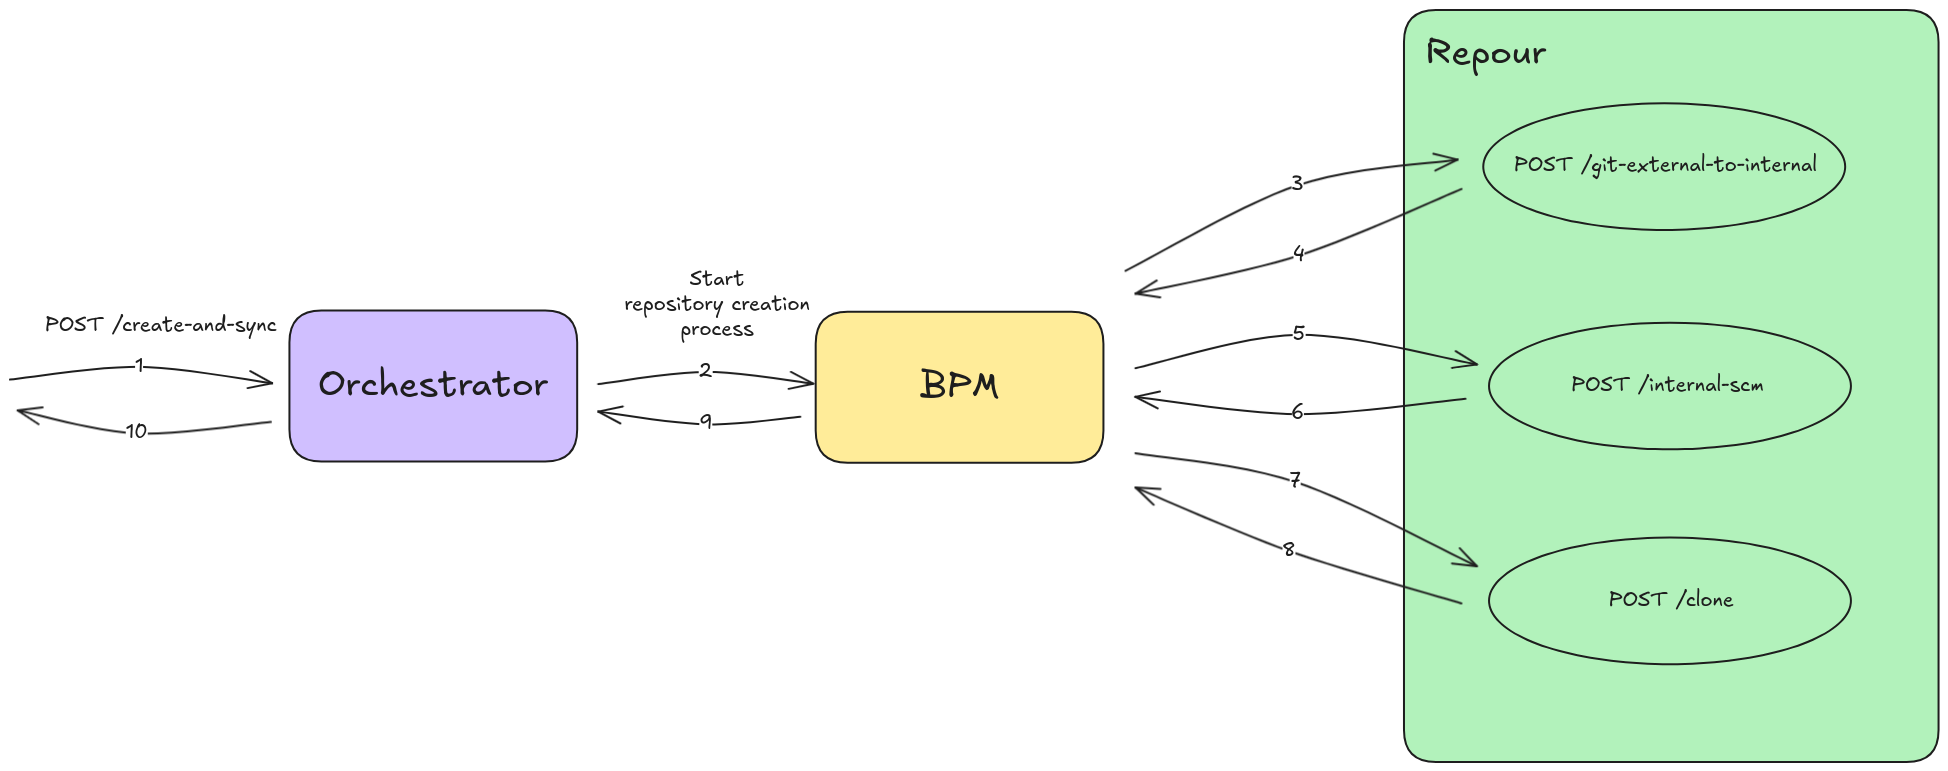
\includegraphics[width=\textwidth]{images/repository-creation-process.png}
  \end{center}
  \caption{Repository creation process}
  \label{fig:repository-creation-process}
\end{figure}

Visual representation of the repository creation process is depicted in Figure \ref{fig:repository-creation-process}.

\end{document}
